\section*{Dati e risultati}

\begin{SCfigure}[1][t!]
	\centering
	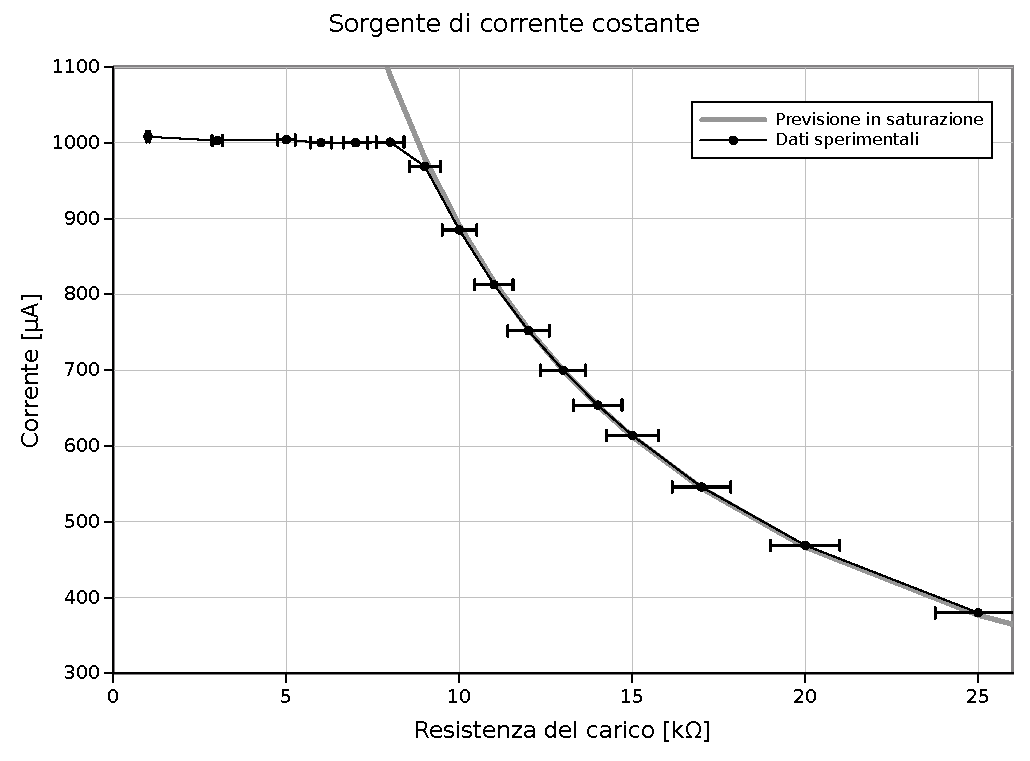
\includegraphics[width=0.75\textwidth]{current.pdf}
	\caption{}
	\label{fig:curr}
\end{SCfigure}

\subsection*{Sorgente di corrente costante}

In questa prima parte dell'esperienza di laboratorio vogliamo dimensionare e studiare il circuito riportato in Figura \ref{fig:}. Questo circuito è una semplice sorgente di corrente costante. Il circuito ha una tensione in ingresso ($V\ped{in}$) di $\SI{10}{\volt}$. La resistenza di collettore $R_c$ è variabile, mentre quella di emettitore $R_e$ ha un valore di $\SI{1}{\kilo\ohm}$.
Per dimensionare il circuito abbiamo fatto ciò che segue; il ramo del circuito relativo al collettore e quello di emettitore sono percorsi dalla stessa intensità di corrente $\SI{1}{\milli\ampere}$. Quindi conoscendo il valore di $R_e$ sappiamo la differenza di potenziale dell'emettitore ($V_e$) che vale $\SI{1}{\volt}$, grazie alla legge di Ohm. Inoltre sappiamo che tra base ed emettitore vi è una caduta di tensione di altri $\SI{0.6}{\volt}$, pertanto la differenza di potenziale ai capi di $R_2$ sarà di $\SI{1.6}{\volt}$.
Quindi, sapendo questa tensione, per ricavare i valori di $R_1$ e $R_2$ ci siamo serviti della nota relazione per un partitore di tensione, ovvero:

\begin{equation}
	V\ped{out} \,=\, V\ped{in}\cdot\frac{R_2}{R_1+R_2} \qquad\text{da cui si ricava che:}\qquad 8.4\,R_2\,=\,1.6\,R_1
\end{equation}

dove $V\ped{out}$ non è altro che la tensione di base del transistor.
Non ci è rimasto che scegliere un valore grande per $R_1$ come $\SI{100}{\kilo\ohm}$ e otteniamo che $R_2$ deve valere circa $\SI{20}{\kilo\ohm}$. Abbiamo scelto un valore di $R_1$ così grande in quanto lo scopo del circuito è quello di convogliare tutta la corrente nel ramo del collettore in modo da eliminare dissipazioni di potenza, pertanto meno corrente passa attraverso $R_1$ e $R_2$ meglio è.

Infine abbiamo acquisito un grafico della corrente di collettore $I_c$ al variare della resistenza di carico $R_c$. I risultati ottenuti sono illustrati nel grafico in Figura \ref{fig:curr}.

\subsection*{Amplificatore ad emettitore comune}

In questa sezione abbiamo montato e dimensionato il circuito in Figura \ref{fig:ampli}. I requisiti che deve avere il nostro circuito sono quelli di avere una tensione di collettore ($V_0$) di $\SI{10}{\volt}$, una corrente di quiescenza di circa $\SI{1}{\milli\ampere}$ e un guadagno $G$ di $-10$. Inoltre il circuito è alimentato da un segnale in ingresso ($V\ped{in}$) sinusodale di frequenza ($\nu$) $\SI{1}{\kilo\hertz}$.

Noi sappiamo che in regime di quiescenza lungo il ramo collettore-emettitore scorre una corrente di $\SI{1}{\milli\ampere}$. Scegliendo $R_e = \SI{500}{\ohm}$ (questo valore ci permette poi di avere un guadagno $G = -10$), si ha $V_E = 0.5 V$ e $V_B = V_E + 0.6 V  = 1.1 V$, si ha che per ottenere un uscita con un clamping simmetrico si deve avere, in quiescienza, $V\ped{out} = V_B + (V_0 - V_B)/2 \simeq 5.5 V$. Inoltre poichè vogliamo che il guadagno, definito come $G\,=\,-R_c/R_e$, sia di -10 possiamo ricavare grazie alle leggi di Ohm il valore di $R_c = \SI{5}{\kilo\ohm}$. In questo modo risulta che, in quiescienza, $V\ped{out} = 5 V$.

Infine sfruttando le stesse considerazioni fatte nella sezione precedente otteniamo i valori di $R_1$ e $R_2$ che sono risultati essere $R_1=\SI{80}{\kilo\ohm}$ e $R_e=\SI{10}{\kilo\ohm}$.
Infine abbiamo determinato il valore di capacità ($C$) sfruttando la relazione che lo lega alla frequenza di risonanza ($\nu$) del filtro passa-altro formato da $C$ e $R_1$ e $R_2$. Vogliamo che non vengano tagliate le frequenze sopra a qualche Hertz.

\begin{equation}
	C \,=\, \frac{1}{2\,\pi\,\nu\,R\ped{eq}} \qquad\text{da cui si ricava che:}\qquad C \,\simeq\,\SI{160}{\nano\farad}
\end{equation}

dove $R\ped{eq}$ è il parallelo tra le resistenze $R_1$ e $R_2$.
Sfruttando l'osciloscopio ne abbiamo verificato il funzionamento e il risultato ottenuto è riportato in Figura \ref{fig:amp}.

\begin{figure}[t!]
	\centering
	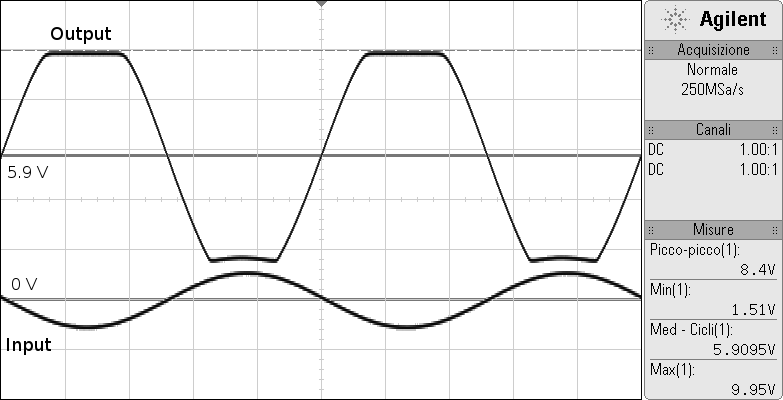
\includegraphics[width=0.75\textwidth]{g.png}
	\caption{Il grafico illustra l'input è l'output dell'amplificatore a emettitore comune. La curva in basso indica l'ingresso $V$,
		che è una sinusoide con VPP = 2 V, mentre la curva in alto la tensione $V\ped{out}$. A lato sono riportati alcuni dati della tensione in uscita.
		Le linee grigie indicano i valor medi delle tendioni. Si nota subito che le tensioni sono
		sfasate di 180$^\circ$, la tensione in uscita è alzata di 5.9 V rispetto all'altra e che il segnale in uscita è amplificato di circa 10 volte.
		Si nota anche il fenomeno del clipping poichè $V\ped{out}$ non può superare i 10 V (linea tratteggiata) e non può scendere sotto 1 V più
		la tensione istantanea della base (segnale in ingresso). Per questo motivo si vede che nella zona di clipping inferiore la d.d.p.
		non è piatta ma segue il profilo della tensione in ingresso.}
	\label{fig:amp}
\end{figure}

\subsection*{Caratteristica in uscita del transistor BC107B}

In questa ultima sezione abbiamo montato il circuito riportato in Figura \ref{fig:transistor}. La resistenza di emettitore $R_e$ ha un valore di $\SI{10}{\ohm}$ mentre la resistenza di base $R_b$ ha un valore di $\SI{100}{\kilo\ohm}$. Abbiamo utilizzato come segnale in ingresso ($V\ped{in}$) un'onda sinusoidale di frequenza ($\nu$) pari a $\SI{1}{\kilo\hertz}$ con una tensione picco-picco di $\SI{10}{\volt}$ ed un offset pari a $+\SI{5}{\volt}$ DC.
Quindi per studiare la caratteristica di uscita del transistor abbiamo utilizzato l'oscilloscopio e abbiamo acquisito tale caratteristica per differenti valori della corrente di base $I_b$ variando la tensione di base ($V_b$). In particolare siamo partiti da una corente minima di base di $\SI{10}{\micro\ampere}$ fino ad arrivare ad una $I_b$ massima di $\SI{90}{\micro\ampere}$ a step di $\SI{10}{\micro\ampere}$.

Il risultato ottenuto è riportato in Figura \ref{fig:cara}.

\begin{SCfigure}[1][t!]
	\centering
	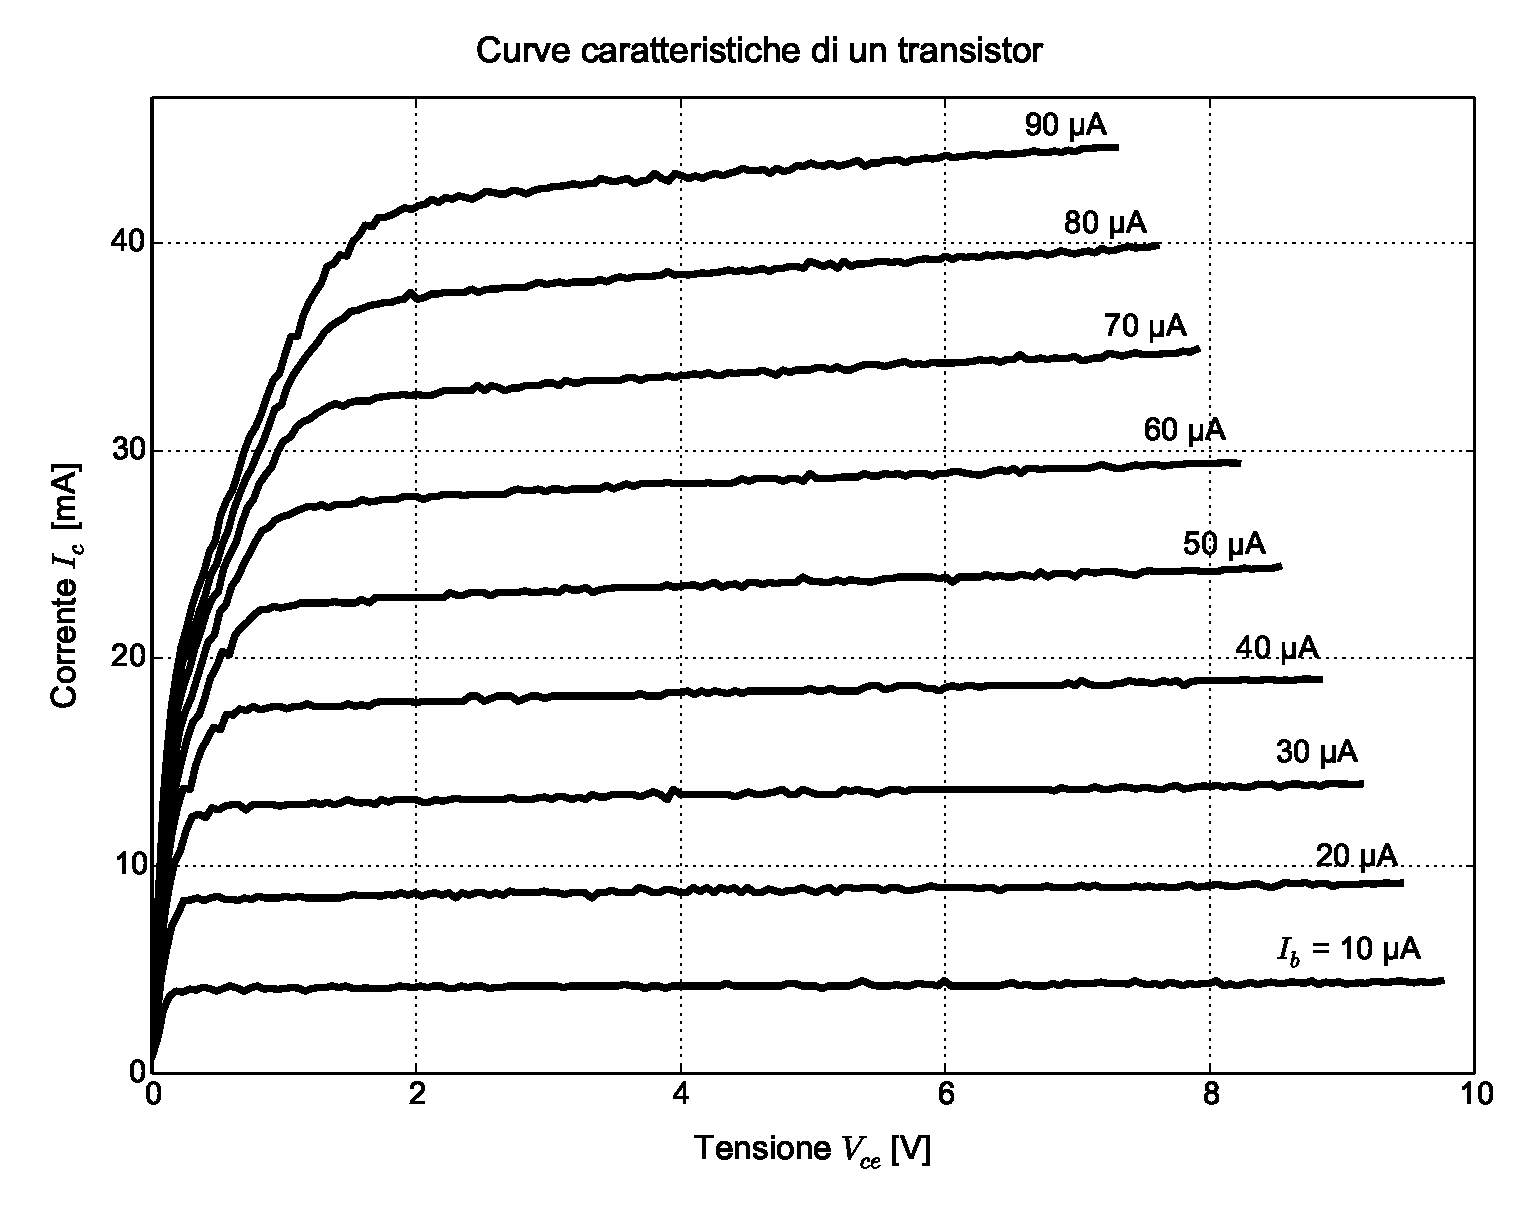
\includegraphics[width=0.75\textwidth]{transistor.pdf}
	\caption{}
	\label{fig:cara}
\end{SCfigure}

Infine abbiamo calcolato per ciascun valore di $I_b$ ilcoefficiente di guadagno in corrente $\beta$ per il valore di tensione di $\SI{5}{\volt}$. Quindi sfruttando la relazione che lega $\beta$ con la corrente di collettore $I_c$ (nota) e la corrente di base $I_b$:

\begin{equation}
	\beta \,=\, \frac{I_c}{I_b}
\end{equation}

abbiamo ottenuto i risultati riportati in Tabella \ref{tab:}.

\begin{table}
    \centering
    \begin{tabular}{l c c}
        \toprule
        &$\beta$ & $\delta\beta$ \\
        \midrule
        & 422 & 6 \\
        & 448 & 5 \\
        & 448 & 5 \\
        & 460 & 5 \\
        & 473 & 5 \\
        & 477 & 5 \\
        & 482 & 5 \\
        & 485 & 5 \\
        & 483 & 5 \\
        \midrule
        Media & 464 & 2 \\
        \bottomrule
    \end{tabular}
\end{table}

